\chapter{Results}

Here is where you discuss the results from your evaluation.
\section{Outputs}
Our program outputs 6 files:\newline
1) The Bathymetry Grid as a heat map\newline
2) The Behavior Grid as a heat map\newline
3) The Goodness Grid as a heat map\newline
4) The Coverage Grid as a heat map\newline
5) The marginal gain in Unique Recovery Rate as a function of the number of receivers placed\newline
6) Text representations of the 5 Grid files, tabular receiver data, and the specified input parameters.\newline
\begin{figure}[h!]
	\label{outputGraphs}
	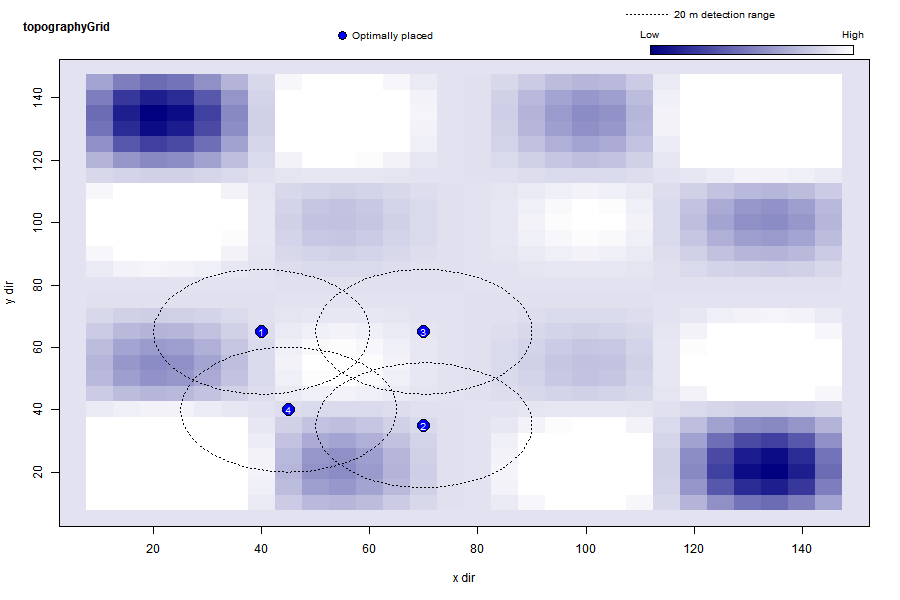
\includegraphics[scale=.5]{TopographyGrid.png}
	\caption{A graphical representation of an artificial Bathymetry file at a 1m resolution (each cell has an edge length of 1m).  Darker cells represent greater depths, while white cells represent inaccessibel terrain (dry land).  The optimal receiver locations are shown on the grid as blue numbered circles, user-placed sensors as grey circles, and projected receivers as green circles.  All receivers have their Detection Range shown as dotted lines.}\label{bathyGraph}
\end{figure}

\begin{figure}[t]
	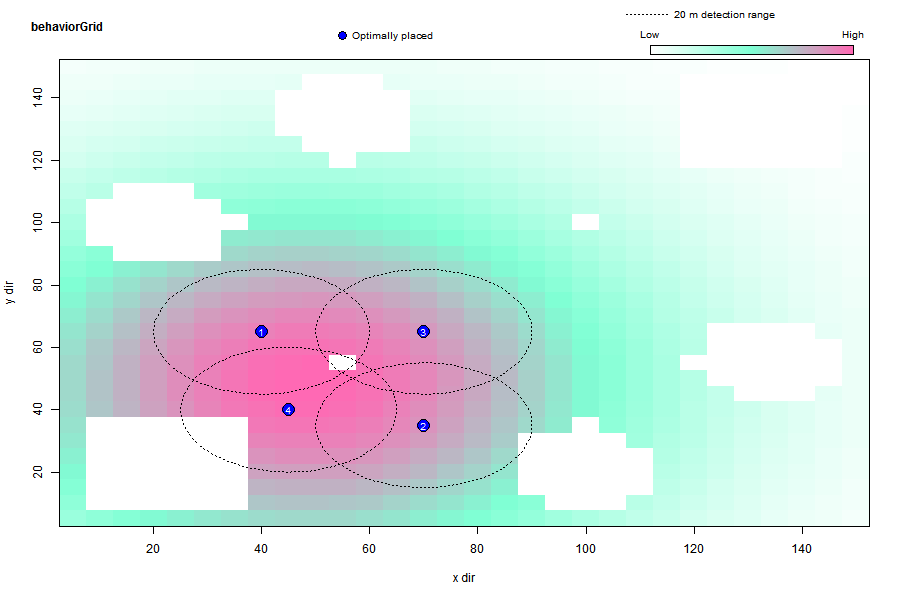
\includegraphics[scale=.5]{BehaviorGrid.png}
	\caption{The Behavior Grid represented as a heatmap.  Higher levels of animal residency correspond with pink cells, moderate levels as light blue, and white for non-residency (ihospitible habitat such as  dry land).  The optimal receiver locations are shown on the grid as blue numbered circles, user-placed sensors as grey circles, and projected receivers as green circles.  All receivers have their Detection Range shown as dotted lines.}\label{animalGraph}
\end{figure}

\begin{figure}[t]
	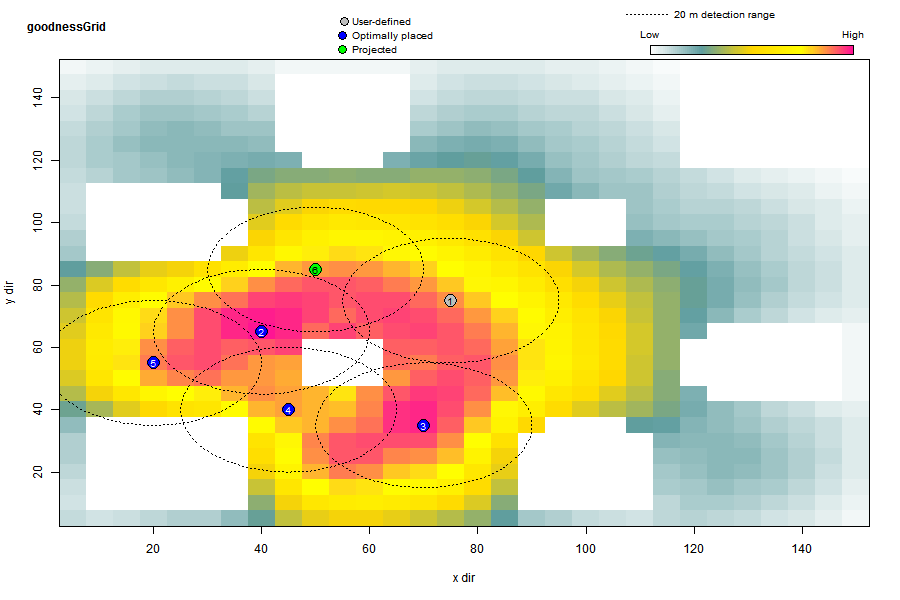
\includegraphics[scale=.5]{GoodnessGrid.png}
	\caption{The Goodness Grid represented as a heatmap showing the quantity of Estimated Receivable Transmissions (ERT) if a receiver were placed in a particular cell.  The legend in the top right assigns color coding to various ERT values. The optimal receiver locations are shown on the grid as blue numbered circles, user-placed sensors as grey circles, and projected receivers as green circles.  All receivers have their Detection Range shown as dotted lines.} \label{goodnessGraph}
\end{figure}

\begin{figure}[t]
	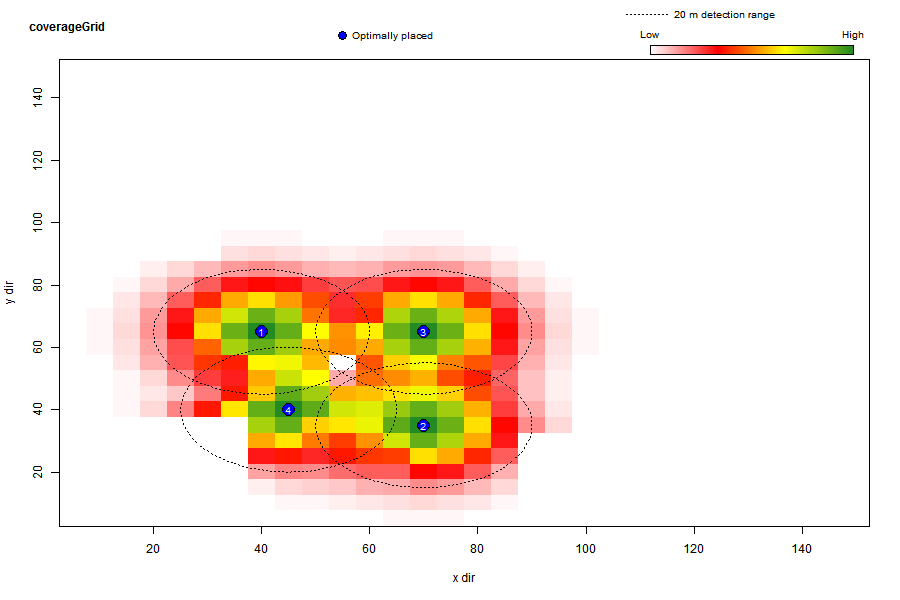
\includegraphics[scale=.5]{CoverageGrid.png}
	\caption{The Coverage Grid represetned as a heatmap showing the quantity of Estimated Receivable Transmissions from each cell in the study site, for the designated reciver array configuration.  The legend in the top right assigns color coding to various ERT values.  The optimal receiver locations are shown on the grid as blue numbered circles, user-placed sensors as grey circles, and projected receivers as green circles.  All receivers have their Detection Range shown as dotted lines.  The missing corner of of Receiver 4's Detection Area is due to the presence of an obscuring section of Bathymetry (dry land).}\label{coverageGraph}
\end{figure}

\begin{figure}[t]
	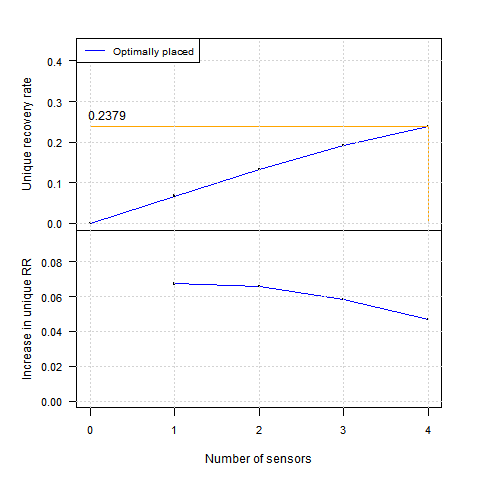
\includegraphics[scale=.8]{RecoveryRates.png}
	\caption{} \label{recoveryGraph}
\end{figure}
\subsection{Grid Graphs}
The four Grid files (Bathymetry, Behavior, Coverage, and Goodness) are visualized as a heat maps.  All of these are overlaid with the resulting receiver locations as numbered circles.  Receiver locations show their detection range as dotted outlines centered over the receiver locations.  User placed receivers are colored white, while receivers placed optimally by the system are colored blue.  The numbering on user and system-placed receivers denotes the rank of each receiver's Unique Data Recovery Rate.  User and system-placed receivers are ranked separately.  Optimal receivers consist both the optimally placed and projected receivers.  The highest ranked receiver locations are returned as the optimal receiver locations, with the lower ranked locations as the projected receiver locations.


\subsection{Data Recovery Graphs}
The program also produces a graph of the marginal increase in and cumulative sum of the Unique Data Recovery Rate as a function of the number of optimally placed receivers used (Figure~\ref{recoveryGraph}).  The graph of the marginal increase in UDRR (the lower graph) is especially useful.  Given that Receivers have a fixed per-unit cost, it makes sense to weigh a receiver's effectiveness (perhaps UDRR contribution) against that cost to determine the utility of purchasing an additional receiver.  The graph of cumulative UDRR is useful to quickly identify the number of receivers necessary to reach a particular UDRR.

\subsection{Text Files}
The program returns a comprehensive text representation of the program output (text dump of gridded data and input parameters), and a short, human-readable document that lists the primary simulation parameters (Evaluation Algorithm, Suppression Algorithm, Behavioral Model, Input Grid Size, and Detection Range), as well as a tabular output of receiver placements (coordinates), data recovery rates for each receiver, and the sparsity of the network.  Projected receivers are excluded from the total UDRR, ADRR, and sparsity values.

Coordinates are returned in both a Global (with respect to the original Topography file) and local (the user specified area of interest) frame.  While the curvature of the earth is well documented, different bathymetric maps may handle the mapping of a 3D curved plane to a 2D grid differently.  For example, one grid may implement some scaling on grid cells a function of the cell's latitude or distance from a certain point.  Other grid files may simply provide non-square grid files.  By proving a small-scale (local) and large-scale (global) frame of reference for our receiver locations, irregularities of this nature are more easily detected.

